

\subsection{Étude de l'hypercube}
Dans cette partie, on va s'intéresser à étudier en détail l'hypercube, objet central de notre mémoire. Cette partie repose sur
l'article wikipedia de l'hypercube \cite{hyp_1} et sur l'article qui résume l'état actuel des connaissances en informatique sur
l'hypercube \cite{hyp_2}. L'hypercube est un graphe beaucoup étudié de part son utilité en informatique, que ce soit le
parallélisme ou bien les codes de Gray. \\

\begin{definition}
    Un code de Gray correspond à un chemin Hamiltonien sur $\mathcal{Q}_n$ vu comme un graphe de retournement
\end{definition}

\begin{definition}
    Un code de Gray cyclique correspond à un cycle hamiltonien sur l'hypercube $\mathcal{Q}_n$ vu comme un graphe de retournement.
    Il y a une correspondance bijective.
\end{definition}

Grâce à cette correspondance avec les graphes, l'analyse des codes de Gray devient une analyse de chemin hamiltonien, plus accessible.
Nous allons particulièrement nous pencher sur les opérations qui préservent l'intégrité des codes de Gray.

On s'intéresse à l'hypercube $\mathcal{Q}_n$ de dimension $n$ car c'est une représentation sous forme de graphe des $2^n$ mots possibles,
quand on les codes avec $n$ bits.

\begin{definition}
    On peut construire $\mathcal{Q}_n$ comme le graphe dont les sommets sont les $2^n$ vecteurs booléens $n$-dimensionnel, autrement
    dit les vecteurs avec des coordonnées binaires, et dont deux sommets sont adjacents si et seulement si les vecteurs ne diffèrent
    que d'une coordonnée.
\end{definition}

Il est aussi possible de construire récursivement $\mathcal{Q}_n$ à partir de deux copies de $\mathcal{Q}_{n-1}$.

\begin{definition}
    Soient deux graphes $G=(V,E)$ et $G'=(V',E')$. Le produit cartésien $H = G \times G'$ est défini comme suit :
    \begin{itemize}
        \item $V(H)=\{(s,s')~|~s\in V,~ s' \in V'\}$
        \item $E(H)=\{e_{\{(u,u'),(v,v')\}}|~( u =v \wedge (u'v'\in E')) \vee (u'=v' \wedge (uv\in E))\}$.
    \end{itemize}
\end{definition}

\begin{definition}
    Le $n$-cube, ou l'hypercube de dimension $n$ noté $\mathcal{Q}_n$ est défini récursivement comme le produit cartésien de deux graphes :
    $$\mathcal{Q}_1 = K_2$$
    $$\mathcal{Q}_n = K_2 \times \mathcal{Q}_{n-1}$$
\end{definition}

\begin{table}[h!]
    \centering
    \begin{tabular}{c}
        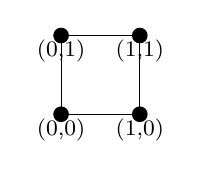
\begin{tikzpicture}
            \foreach \x in {0,1} {
                    \foreach \y in {0,1} {
                            \node at (\x, \y) [circle, fill, inner sep=2pt] {};
                            \node at (\x, \y-0.2) {\footnotesize (\x,\y)};
                        }
                }
            \draw (0,0) -- (1,0);
            \draw (1,0) -- (1,1);
            \draw (1,1) -- (0,1);
            \draw (0,1) -- (0,0);
        \end{tikzpicture}

        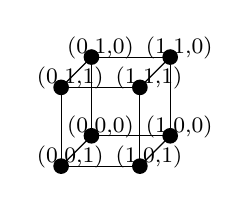
\begin{tikzpicture}
            \foreach \x in {0,1} {
                    \foreach \y in {0,1} {
                            \foreach \z in {0,1} {
                                    \node at (\x, \y, \z) [circle, fill, inner sep=2pt] {};
                                    \node at (\x, \y, \z-0.3) {\footnotesize (\x,\y,\z)};
                                }
                        }
                }
            \foreach \x in {0,1} {
                    \foreach \y in {0,1} {
                            \draw (\x, \y, 0) -- (\x, \y, 1);
                        }
                }
            \foreach \x in {0,1} {
                    \foreach \z in {0,1} {
                            \draw (\x, 0, \z) -- (\x, 1, \z);
                        }
                }
            \foreach \y in {0,1} {
                    \foreach \z in {0,1} {
                            \draw (0, \y, \z) -- (1, \y, \z);
                        }
                }
        \end{tikzpicture}
    \end{tabular}
    \caption{Figure représentant $\mathcal{Q}_2$ et $\mathcal{Q}_3$}
    \label{tab:my_label}
\end{table}
\FloatBarrier

On rappelle les notations qu'un graphe $G=(V, E)$ a $p = |V|$ sommets et $q = |E|$ arêtes, on dit qu'il est d'ordre $p$ et de
taille $q$. Ainsi, $\mathcal{Q}_n$ est d'ordre $2^n$ et de taille $n 2^{n-1}$. \\

On parle de distance, notée $d$, dans un graphe comme le nombre de coordonnées dans lesquels deux vecteurs booléens diffèrent,
par exemple dans $\mathcal{Q}_3$, $d(001, 111) = 2$. Si on considère le graphe comme un graphe de retournement, on parle de
distance de Hamming.

\begin{proposition}
    Le diamètre de $\mathcal{Q}_n$ est $n$, on rappelle que le diamètre est la plus grande distance entre deux paires de sommets.
\end{proposition}

\begin{proposition}
    La somme de toutes les distances entre deux paires de sommets dans $Q_n$, notée $T_d$, est égale à $n 2^{2n-2}$.
\end{proposition}

\begin{preuve}
    On note l'ensemble des sommets de $\mathcal{Q}_n$ par $\{v_1, \cdots, v_p\}$.\\

    On a
    $$T_d(\mathcal{Q}_n) = \underset{1 \leq i < j \leq p}{\sum} d(v_i, v_j)$$

    On partitionne maintenant $\mathcal{Q}_n$ en deux sous-hypercube $\mathcal{Q}_{n-1}$ et $\mathcal{Q}_{n-1}'$. Soit $v_i$ un
    sommet de $\mathcal{Q}_{n-1}$ et $v_i'$ un voisin de $v_i$ dans $\mathcal{Q}_{n-1}'$. On a la distance de $v_i$ à tous les
    sommets de $\mathcal{Q}_n$ qui est égale à

    $$T_{d_i}(\mathcal{Q}_n) := \underset{j}{\sum} d(v_i, v_j)$$

    Maintenant, la distance totale de $v_i$ à tous les sommets de $\mathcal{Q}_{n-1}$ est $T_{d_i}(\mathcal{Q}_{n-1})$ et la
    distance de $v_i$ à un sommet $v_j'$ de $\mathcal{Q}_{n-1}'$ est $d(v_i', v_j')+1$ car $d(v_i, v_i')=1$.\\

    Ainsi la distance totale de $v_i$ aux $2^{n-1}$ sommets de $\mathcal{Q}_{n-1}'$ est
    $$\underset{j}{\sum} (d(v_i', v_j') +1)= T_{d_i}(\mathcal{Q}_{n-1}) + 2^{n-1}$$

    Ce qui implique $T_{d_i}(\mathcal{Q}_n)=2T_{d_i}(\mathcal{Q}_{n-1}) +2^{n-1}$. On vérifie par récurrence sur $n \in \mathbb{N}$
    que $$T_{d_i}(\mathcal{Q}_n) = n 2^{n-1}$$
    Maintenant $\underset{i}{\sum} T_{d_i}(\mathcal{Q}_n)=2^n T_{d_i}(\mathcal{Q}_n) = 2T_d(\mathcal{Q}_n)$ et finalement,
    $$T_d(\mathcal{Q}_n) = n 2^{2n-2}$$
\end{preuve}

\begin{proposition}
    La distance moyenne dans $\mathcal{Q}_n$ est $\partial(\mathcal{Q}_n) = \frac{n 2^{n-1}}{2^n-1}$
\end{proposition}

\begin{preuve}
    On divise la somme de toutes les distances par $\binom{p}{2}$ où $p$ est le nombre de sommet du graphe, ici $p = 2^n$.\\

    On a $\binom{2^n}{2} = \frac{(2^n)!}{(2^n-2)!2!} = \frac{(2^n)(2^n-1)(2^n-2)!}{(2^n-2)!2!} =  2^{n-1} \times (2^n-1)$.\\

    Ainsi, $$\partial(\mathcal{Q}_n) = \frac{T_d(Q_n)}{\binom{2^n}{2}} = \frac{n 2^{2n-2}}{2^{n-1} \times (2^n-1)} = \frac{n 2^{n-1}}{2^n-1}$$
\end{preuve}

On remarque que quand $n$ devient grand, ce ratio se rapproche de $\frac{n}{2}$. \newline

\begin{proposition}
    Les assertions suivantes sont équivalentes :
    \begin{itemize}
        \item Pour tout $n \in \mathbb{N}^*$, $\mathcal{Q}_n$ est $2$-coloriable, son nombre chromatique est $2$.
        \item Pour tout $n \in \mathbb{N}^*$, $\mathcal{Q}_n$ ne possède pas de cycles impair.
        \item Pour tout $n \in \mathbb{N}^*$, $\mathcal{Q}_n$ est biparti.
    \end{itemize}
\end{proposition}

Ces assertions sont équivalentes quelque soit le graphe considéré. Ces points peuvent se démontrer en utilisant la construction
récursive de $\mathcal{Q}_n$, ou d'un point de vue différent en considérant $\mathcal{Q}_n$ comme un graphe de retournement, étant
trivial que ces assertions soient équivalentes, on va juste montrer que $\mathcal{Q}_n$ est biparti.

\begin{preuve}
    Tous les sommets de $\mathcal{Q}_n$ sont de degré $n>0$. Les deux ensembles $A=\{\#1$ dans $v$ est pair $\}$ et $B=\{\#1$ dans
    $v$ est impair$\}$ forment une bipartition de $\mathcal{Q}_n$. Il est rapide de vérifier que pour $v_1, v_2 \in A$
    (resp. $v_1, v_2 \in B$), $d(v_1, v_2) \geq 2$ et donc $v_1v_2$ n'est pas une arête de $\mathcal{Q}_n$. Ce n'est pas un biparti complet.
\end{preuve}

\begin{proposition}
    Pour tout $n \in \mathbb{N}^*$, $\mathcal{Q}_n$ est Hamiltonien.
\end{proposition}

Cette proposition peut se montrer par récurrence sur $n \in \mathbb{N}$ en voyant $\mathcal{Q}_n$ non plus comme un graphe de retournement
mais comme la construction récursive de deux hypercubes de dimensions $n-1$.\\

Un code de Gray cyclique est un cycle hamiltonien sur $\mathcal{Q}_n$. Comme $\mathcal{Q}_n$ est hamiltonien, cela signifie que pour
tout $n \in \mathbb{N}$, il existe un code de Gray cyclique sur des mots binaires de longueur $n$. \\

En général, $\mathcal{Q}_n$ ne possède pas un seul chemin Hamiltonien, ainsi il n'existe pas un unique codage de Gray pour $n$ fixé.
Voici par exemple un tableau donnant le nombre de chemins Hamiltonien en fonction de $n$. On détaillera la notion de cycles isomorphes
plus tard.

\begin{table}[h]
    \centering
    \begin{tabular}{|c|c|c|}
        \hline
        n   & Sans compter les cycles isomorphes & En comptant tous les cycles \\ \hline
        $2$ & $1$                                & $1$                         \\ \hline
        $3$ & $1$                                & $6$                         \\ \hline
        $4$ & $9$                                & $1344$                      \\ \hline
        $5$ & $275065$                           & $906~545~760$               \\ \hline
    \end{tabular}
    \caption{Nombre de cycle Hamiltoniens}
    \label{tab:my_label}
\end{table}

Pour $n \geq 6$ ces valeurs ne sont pas connues. \newline

Le chemin Hamiltonien de $\mathcal{Q}_1$ et le cycles hamiltoniens de $\mathcal{Q}_2$ et $\mathcal{Q}_3$ sont représenté en rouge.

\begin{table}[!h]
    \begin{tabular}{|p{5cm}|c|} \hline
        Code de Gray associé                                                                                                   & Hypercube                                                                                     \\ \hline

        $0 \rightarrow 1$                                                                                                      &
        \begin{tikzcd}
            0 & 1
            \arrow[no head, from=1-1, to=1-2]
            \arrow[color={rgb,255:red,214;green,92;blue,92}, curve={height=6pt}, dashed, no head, from=1-1, to=1-2]
        \end{tikzcd}                                                                                                               \\ \hline

        $00 \rightarrow 10 \rightarrow 11 \rightarrow 01$                                                                      &
        \begin{tikzcd}
            00 & 10 \\
            01 & 11
            \arrow[no head, from=1-1, to=1-2]
            \arrow[color={rgb,255:red,214;green,92;blue,92}, curve={height=6pt}, dashed, no head, from=1-1, to=1-2]
            \arrow[no head, from=1-1, to=2-1]
            \arrow[no head, from=2-1, to=2-2]
            \arrow[no head, from=2-2, to=1-2]
            \arrow[color={rgb,255:red,214;green,92;blue,92}, curve={height=6pt}, dashed, no head, from=1-2, to=2-2]
            \arrow[color={rgb,255:red,214;green,92;blue,92}, curve={height=6pt}, dashed, no head, from=2-2, to=2-1]
            \arrow[color={rgb,255:red,214;green,92;blue,92}, curve={height=6pt}, dashed, no head, from=2-1, to=1-1]
        \end{tikzcd}                                                                                                              \\ \hline

        $000 \rightarrow 001 \rightarrow 101 \rightarrow 100 \rightarrow 110 \rightarrow  111 \rightarrow 011 \rightarrow 010$ &
        \begin{tikzcd}
            001 &&& 011 \\
            & 101 & 111 \\
            & 100 & 110 \\
            000 &&& 010
            \arrow[no head, from=2-2, to=2-3] \arrow[no head, from=2-2, to=3-2]
            \arrow[no head, from=3-2, to=3-3] \arrow[no head, from=3-3, to=2-3]
            \arrow[color={rgb,255:red,214;green,92;blue,92}, curve={height=6pt}, dashed, no head, from=2-3, to=3-3] \arrow[color={rgb,255:red,214;green,92;blue,92}, curve={height=6pt}, dashed, no head, from=3-3, to=3-2]
            \arrow[color={rgb,255:red,214;green,92;blue,92}, curve={height=6pt}, dashed, no head, from=3-2, to=2-2] \arrow[no head, from=2-2, to=1-1]
            \arrow[no head, from=1-1, to=4-1] \arrow[no head, from=4-1, to=3-2]
            \arrow[no head, from=4-1, to=4-4] \arrow[no head, from=4-4, to=3-3]
            \arrow[no head, from=2-3, to=1-4] \arrow[no head, from=1-4, to=1-1]
            \arrow[no head, from=1-4, to=4-4]
            \arrow[color={rgb,255:red,214;green,92;blue,92}, curve={height=6pt}, dashed, no head, from=2-2, to=1-1]
            \arrow[color={rgb,255:red,214;green,92;blue,92}, curve={height=6pt}, dashed, no head, from=1-1, to=4-1]
            \arrow[color={rgb,255:red,214;green,92;blue,92}, curve={height=6pt}, dashed, no head, from=4-1, to=4-4]
            \arrow[color={rgb,255:red,214;green,92;blue,92}, curve={height=6pt}, dashed, no head, from=4-4, to=1-4]
            \arrow[color={rgb,255:red,214;green,92;blue,92}, curve={height=6pt}, dashed, no head, from=1-4, to=2-3]
        \end{tikzcd} \\ \hline
    \end{tabular}
    \caption{Un code de Gray sur $n$ bits associé à un cycle Hamiltonien dans $\mathcal{Q}_n$}
    \label{tab:my_label}
\end{table}
\FloatBarrier

Dans ce mémoire, nous allons principalement nous concentrer sur l'analyse de $\mathcal{Q}_5$, étant donné que les codes de
Beckett-Gray sont disponibles pour tout $n\geq5$. Nous aborderons brièvement le cas $n=6$, bien que les temps de calcul soient
considérablement plus longs dans ce cas. Le diamètre de $\mathcal{Q}_5$ (resp. $\mathcal{Q}_6$ est de $5$ (resp. $6$), son
ordre est de $32$ (resp. $64$) et sa taille est de $80$ (resp. $192$), chaque sommet de $\mathcal{Q}_5$
(resp. $\mathcal{Q}_6$) a un degré de $5$ (resp. $6$), une somme totale de toutes les distances égale à $1280$ (resp. $6144$)
ainsi qu'une distance moyenne entre deux sommets de $2,58$ (resp. $3,04$).
